\addcontentsline{toc}{section}{Appendix}
\section*{\Large Appendix}
\appendix
% Tell TexCount to ignore words in word count
%TC:ignore

\section{Code And Report Source}\label{app:src}
Please find our code and report source here: \url{https://github.com/whattheforkbomb/CM50265/tree/trunk/cw2}
\newpage

\section{Embedding Approach}
\begin{figure}[h!]
    \centering
    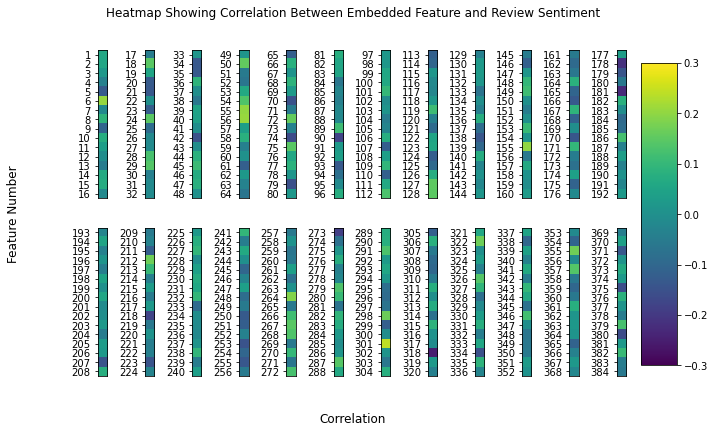
\includegraphics[width=\textwidth]{figures/Feature_Correlation_Heatmap.png}
    \caption{\label{fig:feature_corr_hm_old} Heat-map showing correlation of embedding features to the sentence sentiment with sentence truncation}
\end{figure}
\newpage

\section{SVM Hyper-Parameter Tuning}
\subsection{Polynomial Kernel Hyper-Parameter Grid Search Heatmaps}\label{app:poly_hp}
\begin{figure}[h!]
    \centering
    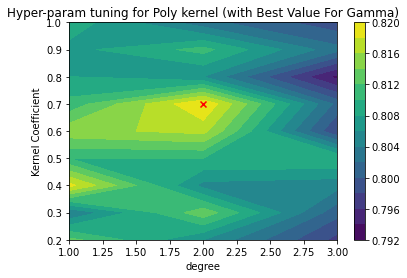
\includegraphics[width=0.6\textwidth]{figures/final/poly_c_d.png}
    \caption{\label{fig:poly_hp_c_d} Contour of Polynomial kernel model hyper-parameter tuning (for C and degree)}
\end{figure}
\begin{figure}[h!]
    \centering
    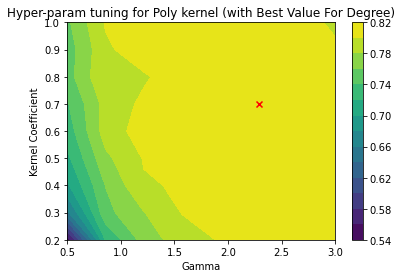
\includegraphics[width=0.6\textwidth]{figures/final/poly_c_g.png}
    \caption{\label{fig:poly_c_g} Heatmap of optimal hyper-parameters C and Gamma for Polynomial Kernel}
\end{figure}
\begin{figure}[h!]
    \centering
    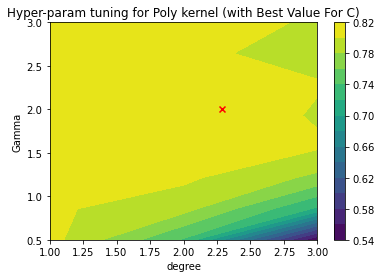
\includegraphics[width=0.6\textwidth]{figures/final/poly_g_d.png}
    \caption{\label{fig:poly_g_d} Heatmap of optimal hyper-parameters Gamma and Degrees for Polynomial Kernel}
\end{figure}
\newpage

\subsection{Linear Kernel Hyper-Parameter Grid Search Heat-Maps}\label{app:lin_hp}
% 'x300', 'x55', 'x5', 'x317', 'x180', 'x177'
\begin{figure}[h!]
    \centering
    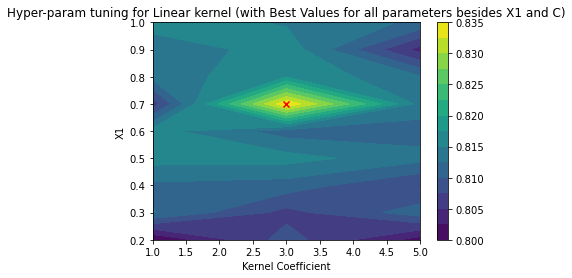
\includegraphics[width=\textwidth]{figures/final/linear_x1.png}
    \caption{\label{fig:lin_300} Heatmap of optimal hyper-parameters C and Weight for feature 300 for Linear Kernel}
\end{figure}
\begin{figure}[h!]
    \centering
    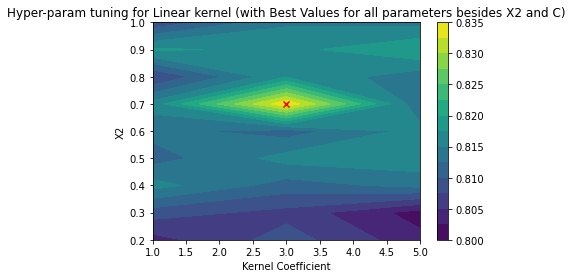
\includegraphics[width=\textwidth]{figures/final/linear_x2.png}
    \caption{\label{fig:lin_55} Heatmap of optimal hyper-parameters C and Weight for feature 55 for Linear Kernel}
\end{figure}
\begin{figure}[h!]
    \centering
    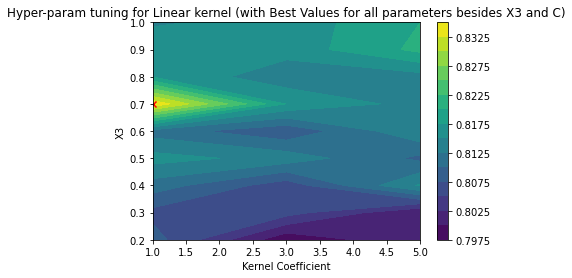
\includegraphics[width=\textwidth]{figures/final/linear_x3.png}
    \caption{\label{fig:lin_5} Heatmap of optimal hyper-parameters C and Weight for feature 5 for Linear Kernel}
\end{figure}
\begin{figure}[h!]
    \centering
    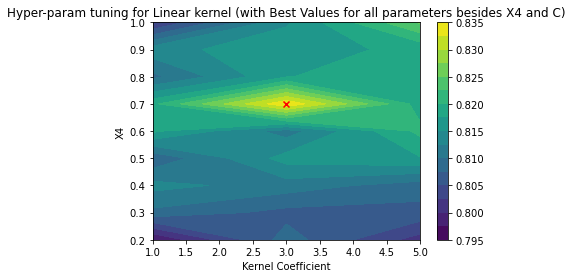
\includegraphics[width=\textwidth]{figures/final/linear_x4.png}
    \caption{\label{fig:lin_317} Heatmap of optimal hyper-parameters C and Weight for feature 317 for Linear Kernel}
\end{figure}
\begin{figure}[h!]
    \centering
    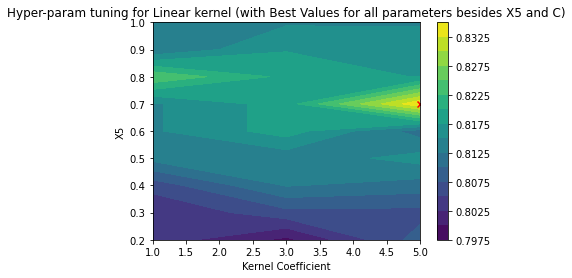
\includegraphics[width=\textwidth]{figures/final/linear_x5.png}
    \caption{\label{fig:lin_180} Heatmap of optimal hyper-parameters C and Weight for feature 180 for Linear Kernel}
\end{figure}
\begin{figure}[h!]
    \centering
    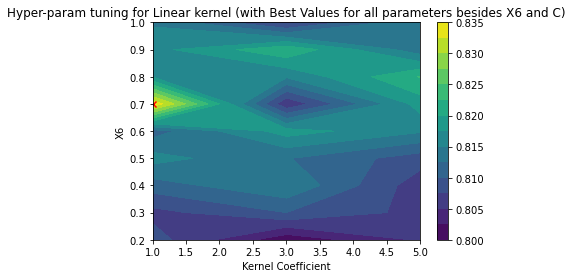
\includegraphics[width=\textwidth]{figures/final/linear_x6.png}
    \caption{\label{fig:lin_177} Heatmap of optimal hyper-parameters C and Weight for feature 177 for Linear Kernel}
\end{figure}
\newpage

\section{SVM Evaluation}\label{app:svm_evaluation}
\subsection{RBF Kernel Model Metrics}
\begin{table}[h!]
    \centering
    \begin{tabular}[h]{c c|c|c|}
        \cline{3-4}
        & & \multicolumn{2}{c|}{Predicted} \\
        \cline{3-4}
        & & + & - \\
        \hline
        \multicolumn{1}{|c|}{\multirow{2}{3em}{Actual}} & + & 744 & 25 \\
        \cline{2-4}
        \multicolumn{1}{|c|}{} & - & 12 & 25 \\
        \hline
    \end{tabular}
    \caption{\label{tab:rbf_confusion}RBF Kernel Model Confusion Matrix}
\end{table}

\begin{table}[h!]
    \centering
    \begin{tabular}[h]{c|c|c|c}
        Classification & Sentence Count & Total Word Count & Average Sentence Length\\
        False Negative & 25 & 7945 & 317.8\\
        False Positive & 12 & 3831 & 319.25\\
        True Negative & 719 & 167818 & 233.4047288\\
        True Positive & 744 & 177046 & 237.9650538\\
    \end{tabular}
    \caption{\label{tab:rbf_wc}RBF Kernel Model impact of sentence length}
\end{table}

\subsection{Polynomial Kernel Model Metrics}
\begin{table}[h!]
    \centering
    \begin{tabular}[h]{c c|c|c|}
        \cline{3-4}
        & & \multicolumn{2}{c|}{Predicted} \\
        \cline{3-4}
        & & + & - \\
        \hline
        \multicolumn{1}{|c|}{\multirow{2}{3em}{Actual}} & + & 747 & 22 \\
        \cline{2-4}
        \multicolumn{1}{|c|}{} & - & 5 & 726 \\
        \hline
    \end{tabular}
    \caption{\label{tab:poly_confusion}Polynomial Kernel Model Confusion Matrix}
\end{table}

\begin{table}[h!]
    \centering
    \begin{tabular}[h]{c|c|c|c}
        Classification & Sentence Count & Total Word Count & Average Sentence Length\\
        False Negative & 22 & 7192 & 326.9090909\\
        False Positive & 5 & 1635 & 327\\
        True Negative & 726 & 170014 & 234.1790634\\
        True Positive & 747 & 177799 & 238.0174029\\
    \end{tabular}
    \caption{\label{tab:poly_wc}Polynomial Kernel Model impact of sentence length}
\end{table}

\subsection{Linear Kernel Model Metrics}
\begin{table}[h!]
    \centering
    \begin{tabular}[h]{c c|c|c|}
        \cline{3-4}
        & & \multicolumn{2}{c|}{Predicted} \\
        \cline{3-4}
        & & + & - \\
        \hline
        \multicolumn{1}{|c|}{\multirow{2}{3em}{Actual}} & + & 663 & 106 \\
        \cline{2-4}
        \multicolumn{1}{|c|}{} & - & 94 & 637 \\
        \hline
    \end{tabular}
    \caption{\label{tab:lin_confusion}Linear Kernel Model Confusion Matrix}
\end{table}

\begin{table}[h!]
    \centering
    \begin{tabular}[h]{c|c|c|c}
        Classification & Sentence Count & Total Word Count & Average Sentence Length\\
        False Negative & 106 & 27228 & 256.8679245\\
        False Positive & 94 & 20946 & 222.8297872\\
        True Negative & 637 & 150703 & 236.5824176\\
        True Positive & 663 & 157763 & 237.9532428\\
    \end{tabular}
    \caption{\label{tab:lin_wc}Linear Kernel Model impact of sentence length}
\end{table}
% Tell TexCount to start counting words again
%TC:endignore
